\section{Descripción del Dataset y Análisis Exploratorio}\label{sec:dataset}

\subsection{Origen y dominio de aplicación}
El conjunto de datos empleado es de acceso \emph{público} y proviene del
repositorio Kaggle bajo el identificador
\texttt{abadpomamaquera/meteorological-data-for-frost-prediction-in-peru}. La
ingesta se realizó de forma programática mediante la librería \texttt{kagglehub}
con el adaptador \texttt{KaggleDatasetAdapter.PANDAS}. El dominio de aplicación
corresponde a la \emph{meteorología agrícola} de las regiones altoandinas del
Perú, y la unidad de observación es un registro meteorológico horario asociado a
estaciones de medición. Según la documentación oficial del repositorio, el
dataset integra variables atmosféricas y geográficas comúnmente asociadas a la
formación de heladas, seleccionadas por su relevancia en estudios agroclimáticos
y ambientales.

El repositorio ofrece dos versiones: \texttt{DATASET.csv}, descrito como el
conjunto completo tras un preprocesamiento inicial, y
\texttt{DATASET\_FILTRADO.csv}, la versión filtrada empleada por el autor
original para entrenar un clasificador XGBoost. El presente trabajo utiliza
deliberadamente la versión \texttt{DATASET.csv} con un clasificador Random Forest,
constituyendo un pipeline de preprocesamiento y modelado independiente del
propuesto por el autor del repositorio, lo que permite un contraste metodológico.

\subsection{Tamaño, instancias y características}
El archivo \texttt{DATASET.csv} ocupa $301.77$\,MB en disco según la
documentación oficial del repositorio. La matriz cargada contiene
$N = 1\,672\,827$ instancias y $D = 18$ características, con una huella real en
memoria de $229.7$\,MB según \texttt{df.info()}. En cuanto a los tipos de dato,
16 variables son de punto flotante (\texttt{float64}) y 2 son enteras
(\texttt{int64}), correspondientes a las variables temporales \texttt{año} y
\texttt{dia}.

\subsection{Observación sobre la calidad de los datos}
Aunque la documentación del repositorio describe \texttt{DATASET.csv} como un
conjunto ``limpio y estandarizado'' del que se habrían removido los registros
faltantes e inconsistentes, el análisis exploratorio realizado en este trabajo
detectó que dicha versión \emph{conserva} el código de error de sensor
\texttt{-999} sin corregir (Fig.~\ref{fig:eda_raw}). Adicionalmente, se identificó
una discrepancia entre la documentación y el contenido efectivo del archivo: la
ficha oficial menciona un ``balance de radiación'' entre las variables, pero el
análisis de las 18 columnas no identifica ninguna variable de radiación; las
columnas efectivamente presentes son las 18 listadas en la Tabla~\ref{tab:dict},
incluyendo coordenadas geográficas (\texttt{latitud}, \texttt{longitud}) y
\texttt{altitud}. Estas observaciones justifican la etapa de corrección de
anomalías descrita en la Sección~\ref{sec:preprocessing} y refuerzan la necesidad
de un diagnóstico independiente de la calidad de los datos, incluso cuando la
fuente los declara preprocesados.

\subsection{Diccionario de variables}
La Tabla~\ref{tab:dict} presenta el diccionario de variables con sus rangos
empíricos reales, obtenidos mediante \texttt{df.describe()}. Se observa que 13 de
las 16 variables continuas presentan un valor mínimo de \texttt{-999},
correspondiente al código de error de sensor; en contraste, las variables
temporales (\texttt{año}, \texttt{dia}) y geográficas (\texttt{latitud},
\texttt{longitud}, \texttt{altitud}) presentan rangos físicamente válidos, lo que
valida la aplicación selectiva del filtro de corrección. Los rangos de
\texttt{latitud} $[-18.01, -8.19]$ y \texttt{longitud} $[-78.04, -69.06]$
confirman geográficamente la procedencia peruana de las estaciones.

\begin{table}[H]
\centering
\caption{Diccionario de variables con rangos empíricos ($N=1\,672\,827$)}
\label{tab:dict}
\scriptsize
\renewcommand{\arraystretch}{1.15}
\begin{tabular}{p{1.9cm}p{0.7cm}p{1.9cm}p{2.2cm}}
\toprule
\textbf{Variable} & \textbf{Tipo} & \textbf{Rango [min, max]} & \textbf{Descripción física} \\
\midrule
\texttt{año} & entera & [2000, 2025] & Año del registro \\
\texttt{dia} & entera & [1, 366] & Día juliano del registro \\
\texttt{temp\_2m} & continua & [-999, 30.21] & Temperatura del aire a 2\,m ($^\circ$C) \\
\texttt{punto\_rocio\_2m} & continua & [-999, 20.84] & Punto de rocío a 2\,m ($^\circ$C) \\
\texttt{temp\_max\_2m} & continua & [-999, 36.77] & Temperatura máxima a 2\,m ($^\circ$C) \\
\texttt{temp\_min\_2m} & continua & [-999, 25.03] & Temperatura mínima a 2\,m; base de la etiqueta \\
\texttt{humedad\_rel\_2m} & continua & [-999, 99.74] & Humedad relativa a 2\,m (\%) \\
\texttt{viento\_2m} & continua & [-999, 7.47] & Velocidad del viento a 2\,m (m/s) \\
\texttt{viento\_max\_2m} & continua & [-999, 11.61] & Ráfaga máxima a 2\,m (m/s) \\
\texttt{viento\_min\_2m} & continua & [-999, 5.57] & Viento mínimo a 2\,m (m/s) \\
\texttt{viento\_10m} & continua & [-999, 10.49] & Velocidad del viento a 10\,m (m/s) \\
\texttt{viento\_max\_10m} & continua & [-999, 15.16] & Ráfaga máxima a 10\,m (m/s) \\
\texttt{viento\_min\_10m} & continua & [-999, 6.98] & Viento mínimo a 10\,m (m/s) \\
\texttt{humedad\_suelo} & continua & [-999, 0.98] & Humedad volumétrica del suelo \\
\texttt{precipitacion} & continua & [-999, 470.24] & Precipitación acumulada (mm) \\
\texttt{latitud} & continua & [-18.01, -8.19] & Latitud de la estación (grados) \\
\texttt{longitud} & continua & [-78.04, -69.06] & Longitud de la estación (grados) \\
\texttt{altitud} & continua & [1079.2, 4691.4] & Altitud de la estación (m.s.n.m.) \\
\midrule
\texttt{Target\_Helada} & binaria & \{0, 1\} & Etiqueta derivada: $1$ si $\texttt{temp\_min\_2m}\le 0^\circ$C \\
\bottomrule
\end{tabular}
\end{table}

\subsection{Distribuciones de las variables densas}
El análisis exploratorio inicial sobre los datos crudos reveló una anomalía
crítica de calidad: prácticamente todas las variables numéricas presentaban una
extensión de su soporte hacia valores físicamente imposibles, cercanos a
$-1000$, que comprimía la distribución real en una línea recta indistinguible
(Fig.~\ref{fig:eda_raw}). Esto evidenció que los sensores codificaron los fallos
de lectura mediante el valor de relleno \texttt{-999}. Tras la corrección
(Sección~\ref{sec:preprocessing}), las funciones de densidad recuperan su
topología termodinámica real (Fig.~\ref{fig:eda_clean}).

\begin{figure}[H]
\centering
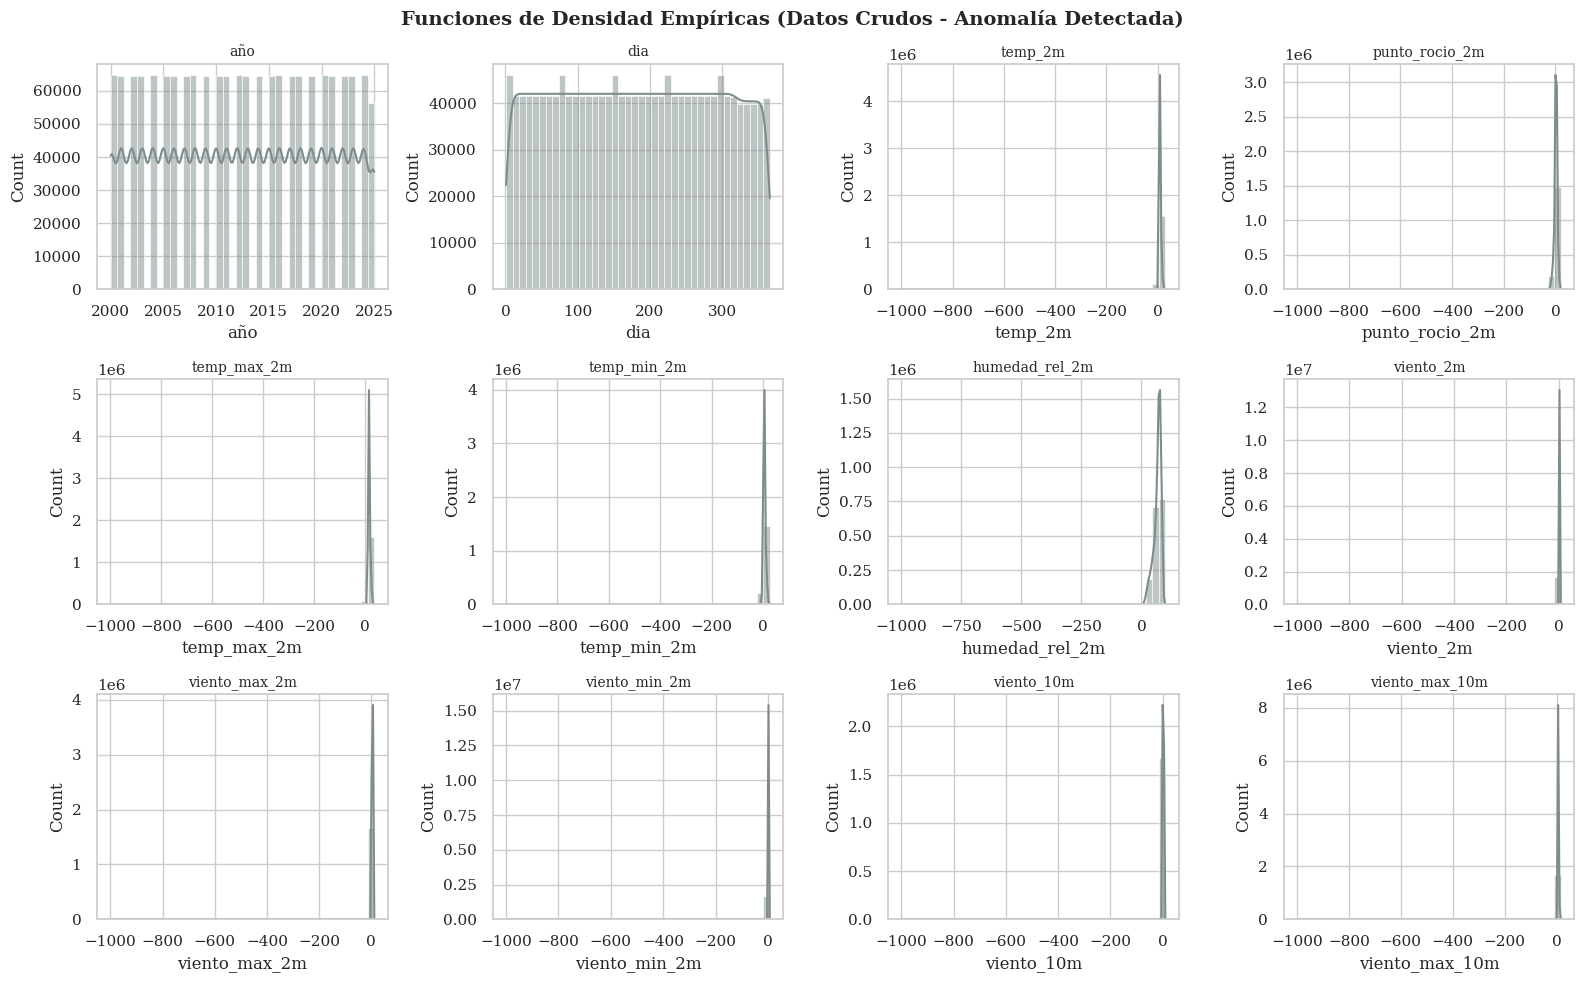
\includegraphics[width=1.00\textwidth]{img/cell4_out0.png}
\caption{Funciones de densidad empíricas sobre los datos crudos. La anomalía de
codificación de error (\texttt{-999}) colapsa las distribuciones reales.}
\label{fig:eda_raw}
\end{figure}

\begin{figure}[H]
\centering
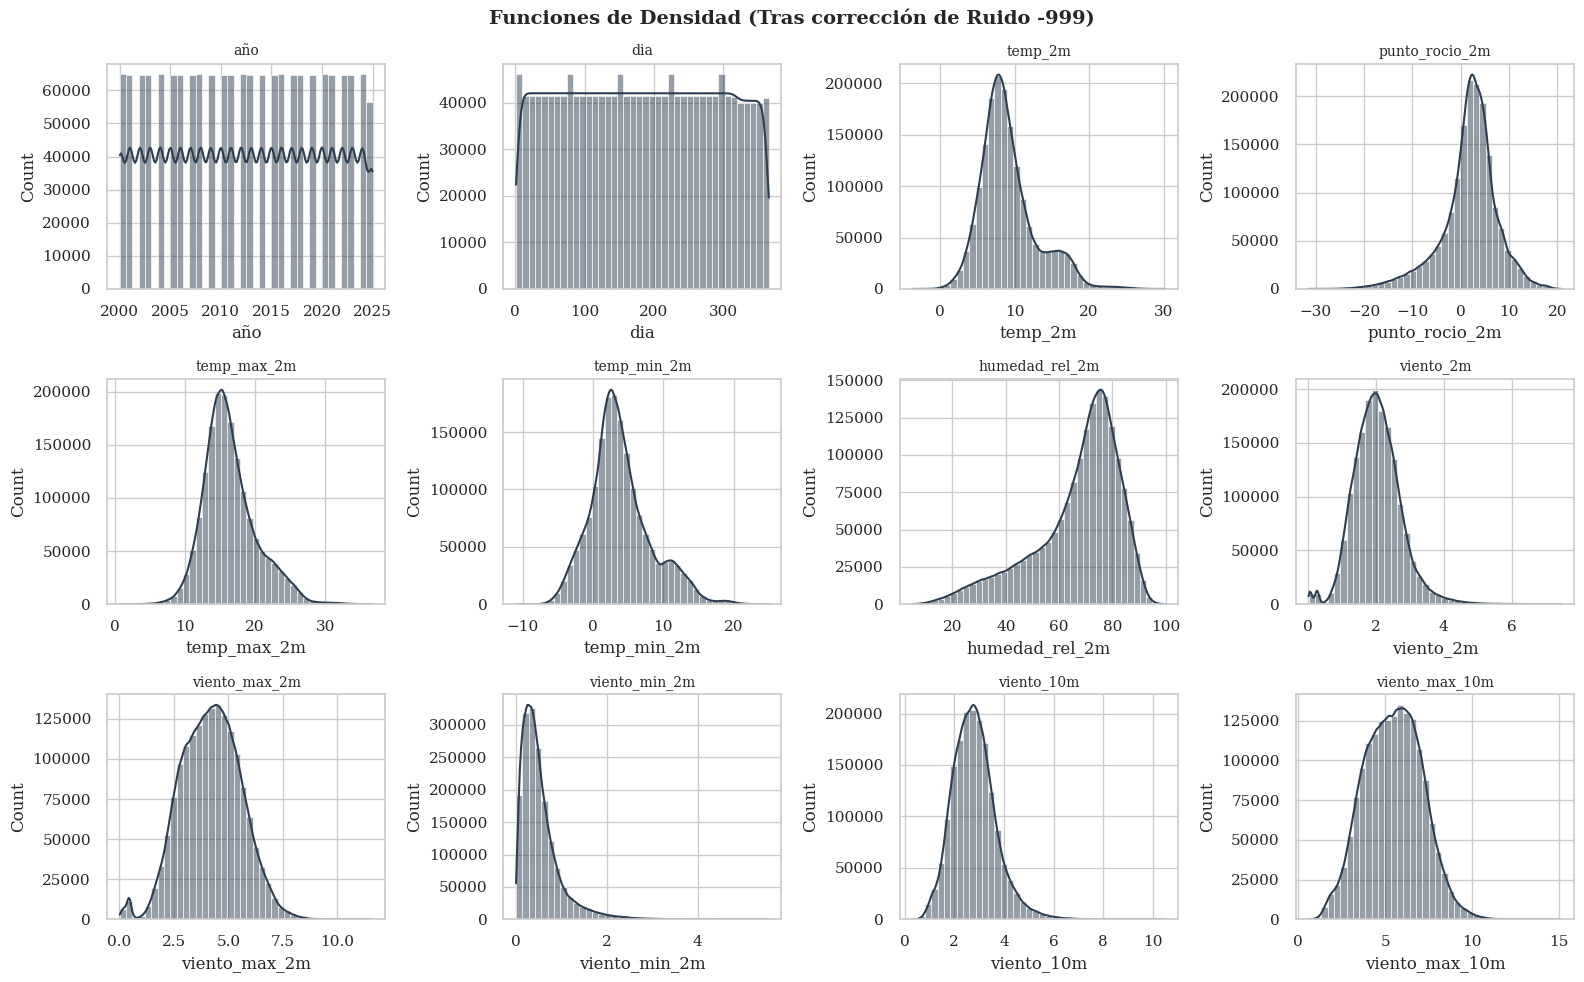
\includegraphics[width=1.00\textwidth]{img/cell6_out1.png}
\caption{Funciones de densidad empíricas tras la corrección del código de error
\texttt{-999}, mostrando la topología real de las variables meteorológicas.}
\label{fig:eda_clean}
\end{figure}

\subsection{Valores faltantes}
Un aspecto metodológicamente relevante es que el archivo original no contiene
valores nulos explícitos: la inspección estructural (\texttt{df.info()}) reporta
$1\,672\,827$ registros no nulos en las 18 columnas. Los datos faltantes se
encontraban \emph{enmascarados} bajo el código de error \texttt{-999}, y solo
emergen como nulos tras aplicar el filtro de corrección descrito en la
Sección~\ref{sec:preprocessing}. Una vez desenmascarados, la verdadera tasa de
datos faltantes resulta baja y homogénea: exactamente 531 registros por variable
numérica afectada, equivalentes al $0.031743\%$ del total
(Tabla~\ref{tab:missing}). Esta uniformidad sugiere un origen común de los fallos
de sensor, probablemente ventanas de mantenimiento o cortes simultáneos de
adquisición. La detección de este enmascaramiento constituye precisamente la
justificación de la etapa de corrección de anomalías, dado que un diagnóstico
superficial basado únicamente en \texttt{df.info()} habría concluido erróneamente
que el conjunto estaba libre de datos faltantes.

\begin{table}[H]
\centering
\caption{Tasa de valores faltantes tras desenmascarar el código de error}
\label{tab:missing}
\footnotesize
\begin{tabular}{lcc}
\toprule
\textbf{Variables afectadas} & \textbf{Faltantes} & \textbf{Porcentaje} \\
\midrule
13 variables numéricas & 531 c/u & $0.031743\%$ \\
\bottomrule
\end{tabular}
\end{table}

\subsection{Desbalance severo de clases}
El análisis de la variable objetivo confirmó un desbalance de clases agudo, un
problema crítico para el modelado posterior (Tabla~\ref{tab:imbalance}). La clase
de interés (ocurrencia de helada) representa apenas el $16.24\%$ de las
observaciones, lo que justifica el uso de ponderación balanceada de clases y de
métricas robustas al desbalance en lugar de la exactitud.

\begin{table}[H]
\centering
\caption{Distribución de la variable objetivo \emph{Target\_Helada}}
\label{tab:imbalance}
\footnotesize
\begin{tabular}{lcc}
\toprule
\textbf{Clase} & \textbf{Instancias} & \textbf{Porcentaje} \\
\midrule
0 (Normal) & 1\,401\,118 & $83.757496\%$ \\
1 (Helada) & 271\,709 & $16.242504\%$ \\
\midrule
\textbf{Total} & \textbf{1\,672\,827} & $100\%$ \\
\bottomrule
\end{tabular}
\end{table}

\subsection{Correlación lineal (Pearson)}
Se calculó la matriz de correlación lineal de Pearson sobre una submuestra de
$\min(N, 20\,000)$ registros completos, con semilla fija ($\text{SEED}=42$),
visualizada mediante un mapa de calor con máscara triangular superior
(Fig.~\ref{fig:corr}). Las cinco variables con mayor correlación lineal absoluta
respecto a la helada fueron \texttt{punto\_rocio\_2m} ($r=0.5581$),
\texttt{temp\_2m} ($r=0.4867$), \texttt{altitud} ($r=0.3779$),
\texttt{humedad\_rel\_2m} ($r=0.3007$) y \texttt{temp\_max\_2m} ($r=0.2856$). El
mapa evidencia además alta multicolinealidad entre grupos de sensores
relacionados (variantes de viento y de temperatura), lo que motiva la reducción
de dimensionalidad mediante PCA.

\begin{figure}[H]
\centering
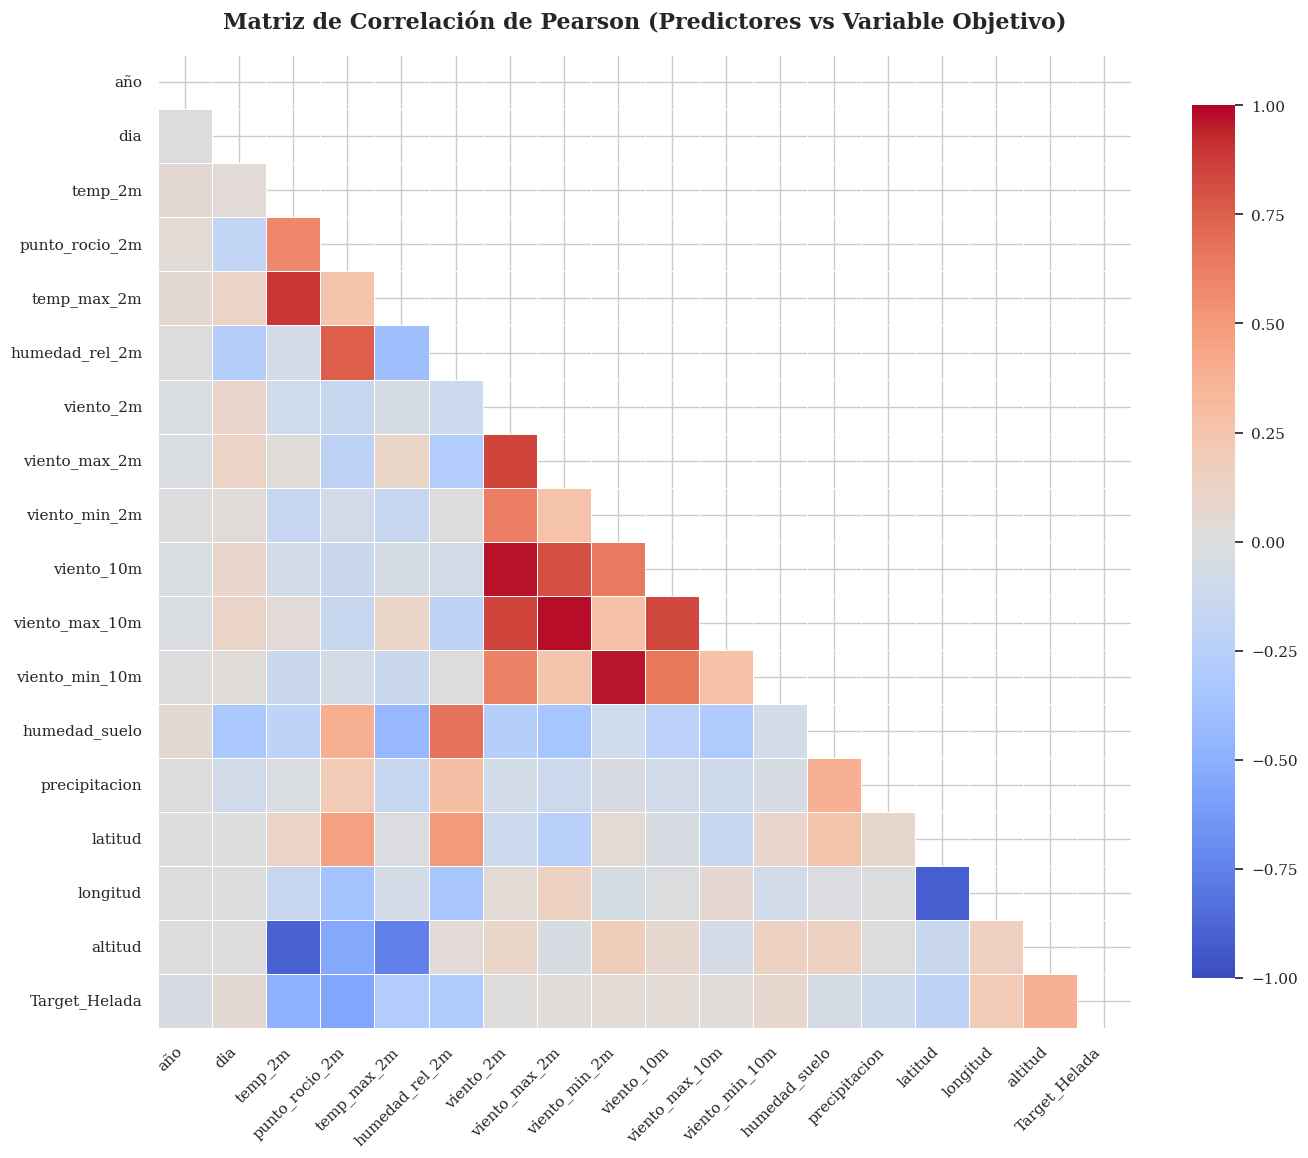
\includegraphics[width=1.00\textwidth]{img/cell8_out2.png}
\caption{Matriz de correlación lineal de Pearson entre predictores y la variable
objetivo \emph{Target\_Helada}.}
\label{fig:corr}
\end{figure}

\subsection{Valores atípicos univariados legítimos}
Más allá del artefacto \texttt{-999}, el análisis de los estadísticos descriptivos
revela un valor atípico físicamente legítimo en la variable
\texttt{precipitacion}: su máximo alcanza $470.24$\,mm frente a un tercer cuartil
de apenas $0.87$\,mm y una mediana de $0.04$\,mm (Tabla~\ref{tab:dict}). Este
valor no constituye un error de sensor sino un evento de precipitación extrema
real. Coherentemente con el tratamiento adoptado para las heladas, tales extremos
se preservan como señal y se protegen mediante el escalamiento robusto
(\texttt{RobustScaler}) descrito en la Sección~\ref{sec:preprocessing}, en lugar
de eliminarse.

\subsection{Correlación no lineal y outliers multivariados}
El pipeline analizado no computa una matriz de correlación no lineal: el
coeficiente de Spearman fue descartado explícitamente bajo el supuesto de
relaciones lineales paramétricas para la posterior reducción vía PCA. De igual
forma, no se aplicó detección de outliers multivariados (p.\,ej. \emph{Isolation
Forest} o \emph{LOF}), dado que los valores climáticos extremos se interpretan
como precursores físicos legítimos del evento de helada y no como ruido; el único
artefacto anómalo tratado fue el código de error univariado \texttt{-999}. La
incorporación de medidas de dependencia no lineal (correlación de Spearman o
información mutua) y de detección de anomalías multivariadas se plantea como
línea de trabajo futuro.